\begin{figure}[t]
    \centering
    \begin{subfigure}[b]{0.8\linewidth}
        \centering
        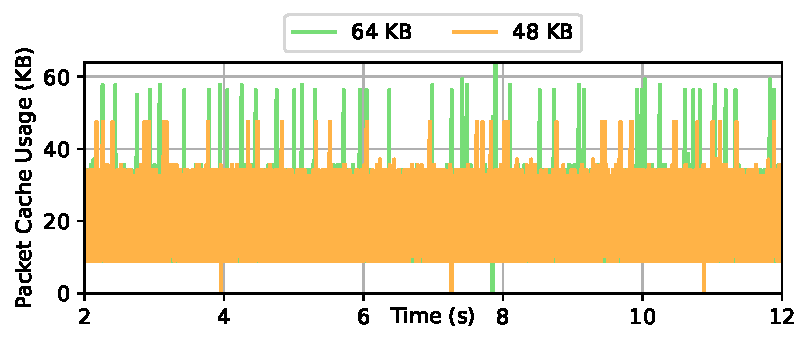
\includegraphics[width=\linewidth]{figures/cache_http.pdf}
        \caption{HTTP/3 file download.
        % \thea{May be a non-issue, but not sure how to interpret the mass of orange here.}
        }
        \label{fig:memory:http}
    \end{subfigure}
    \begin{subfigure}[b]{0.8\linewidth}
        \centering
        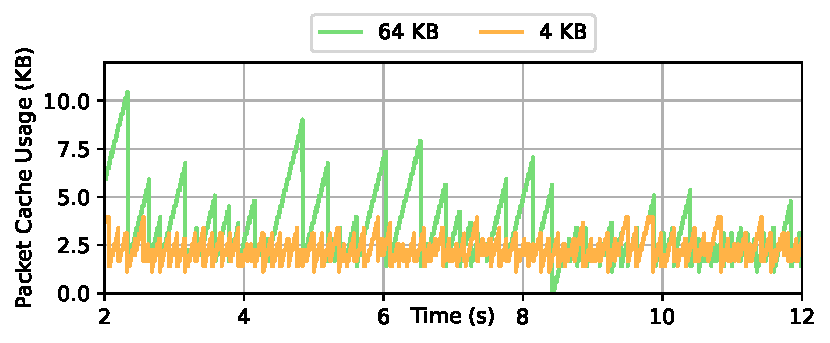
\includegraphics[width=\linewidth]{figures/cache_media.pdf}
        \caption{Low-latency media with FEC.}
        \label{fig:memory:media}
    \end{subfigure}
    \caption{\small The number of bytes in the cache over a
     10-second period with both bounded (48 KB or 4 KB) and unbounded (64 KB)
     cache sizes. The proxy uses optimistic eviction if an incoming packet
     causes the cache to exceed its capacity.}
    \label{fig:memory}
\end{figure}

\begin{figure}[t]
    \centering
    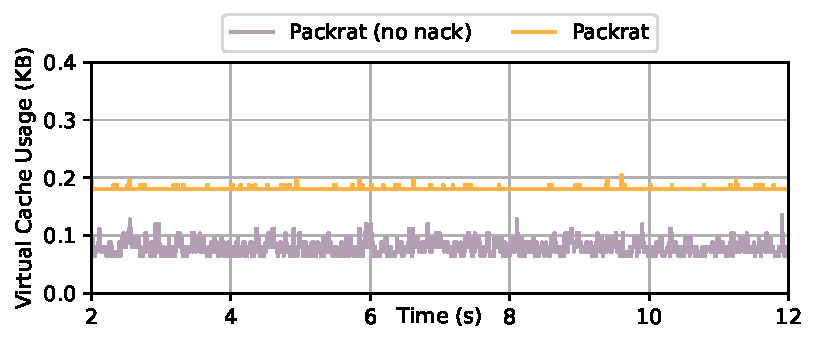
\includegraphics[width=0.8\linewidth]{figures/cache_multicast.pdf}
    \caption{The sum of the virtual cache sizes of all $16$ clients in
     the multicast application. Each client uses $\approx\!$12 bytes each for a
     single insertion pair. The variations are due to individuals having
     slightly more or less than one insertion pair. Without selective eACKing
     (``no nack''), clients more often have empty virtual buffers. The base
     connection's packet cache (not pictured) is always 64 KB.}
    \label{fig:memory:multicast}
\end{figure}